\documentclass{beamer}
\mode<presentation> {
    \usetheme{Copenhagen} \usecolortheme{whale}
    }
\usepackage{graphicx}
\usepackage{multicol}
\setbeamersize{text margin left=3mm,text margin right=5mm}

\graphicspath{{Images/}}

\title[Assignments 3]{I\&I Stimatore di Frequenza}
\author{Lorenzo Rossi Matricola: 0301285}
\begin{document}
\begin{frame}
	\titlepage{}
\end{frame}
\begin{frame}
	\begin{columns}[t]
		\begin{column}{.5\textwidth}
			\tableofcontents[sections={1-3}] % chktex 8
		\end{column}
		\begin{column}{.5\textwidth}
			\tableofcontents[sections={4-5}] % chktex 8
		\end{column}
	\end{columns}
\end{frame}
\begin{frame}
    \frametitle{Assignment 3}
    \section{Introduzione}
    Considerati i segnali:\begin{equation*}
        y_1(t)=\sin{100 t}\quad y_2(t)=\sin(t)
    \end{equation*}
    Implementare il metodo di stima di frequenza I\&I verificandone l'efficacia e discuti quale è una buona scelta del guadagno k.\newline Inoltre, i segnali misurati sono affetti dal disturbo additivo \begin{equation*}
        d=0.001 \sin{50 t}
    \end{equation*}
\end{frame}
\begin{frame}
    \frametitle{Modello Teorico}
    \section{Modello Teorico}
    \begin{itemize}
        \item \textbf{Dinamica:}\begin{align*}
            \dot{\hat{x}}=-k_{1}*\hat{x}-y,\quad\quad \dot{\hat{\theta_{1}}}=\Delta(y,\hat{x},\hat{\theta_{1}})=y^2-k_{1}\hat{x}^2-y\hat{x}^3-\hat{\theta_{1}}\hat{x}^3
        \end{align*}
        \item \textbf{Dinamica Erorre:}
        \begin{align*}
            \dot{z_{x}}=-k_{1}z_{x},\quad\quad \dot{z_{\theta}}=-\hat{x}-\hat{x}^{2}z_{\theta}\\
        \end{align*}
        con \(k_{1}>0\)
        \item \textbf{Stime:}
         \begin{align*}
            &\text{Frequenza:}\theta_{est}=y\hat{x}+\hat{\theta_{1}}\\
            &\text{ Stima di x:} x_{est}=k_{1}y+\hat{x}(k_{1}^{2}+\theta_{est})
        \end{align*}
    \end{itemize}
\end{frame}
\begin{frame}
    \frametitle{Simulink - 1}
    \section{Implementazione Simulink}
    \subsection{Dinamica 1}
    \begin{itemize}
        \item \textbf{Dinamica}
    \end{itemize}
    \begin{minipage}[t]{0.9\textwidth}
        \begin{equation*}
            \dot{\hat{x}}=-k_{1}\hat{x}-y
        \end{equation*}
        \begin{figure}
            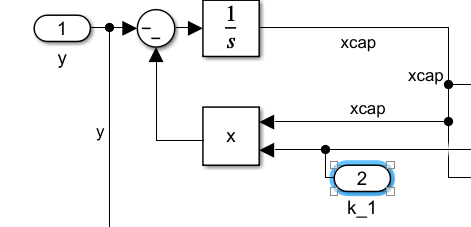
\includegraphics[scale=0.4]{2022-05-15-17-24-30.png} %chktex 8
        \end{figure}
    \end{minipage}
\end{frame}
\begin{frame}
    \frametitle{Simulink - 2} %chtex 8
    \subsection{Dinamica 2}
    \begin{itemize}
        \item \textbf{Dinamica 2}
    \end{itemize}
    \begin{minipage}[t]{0.9\textwidth}
        \begin{equation*}
            \dot{\hat{\theta_{1}}}=y^2-k_{1}\hat{x}^2-y\hat{x}^3-\hat{\theta_{1}}\hat{x}^2
        \end{equation*}
        \begin{figure}
            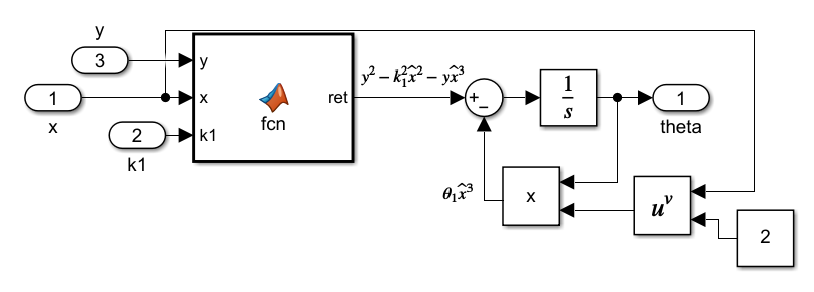
\includegraphics[scale=0.3]{2022-05-15-17-59-30.png} %chktex 8
        \end{figure}
    \end{minipage}
\end{frame}
\begin{frame}
    \frametitle{Simulink - 3} %chtex 8
    \subsection{Dinamica Errore}
    \begin{itemize}
        \item \textbf{Dinamica Errore}
    \end{itemize}
    \begin{minipage}[t]{0.9\textwidth}
        \begin{figure}
            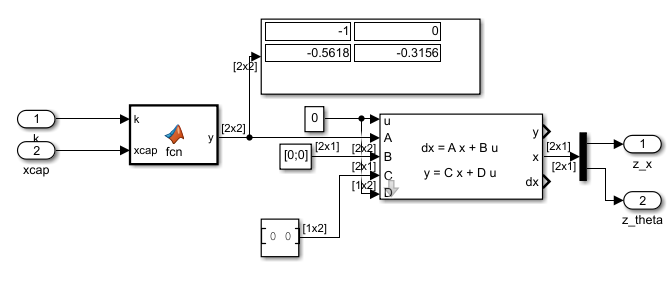
\includegraphics[scale=0.4]{2022-05-15-17-53-20.png} %chktex 8
        \end{figure}
    \end{minipage}
\end{frame}
\begin{frame}
    \frametitle{Simulink - 4} %chtex 8
    \subsection{Stima}
    \begin{itemize}
        \item \textbf{Stima}
    \end{itemize}
    \begin{minipage}[t]{0.9\textwidth}
        \begin{figure}
            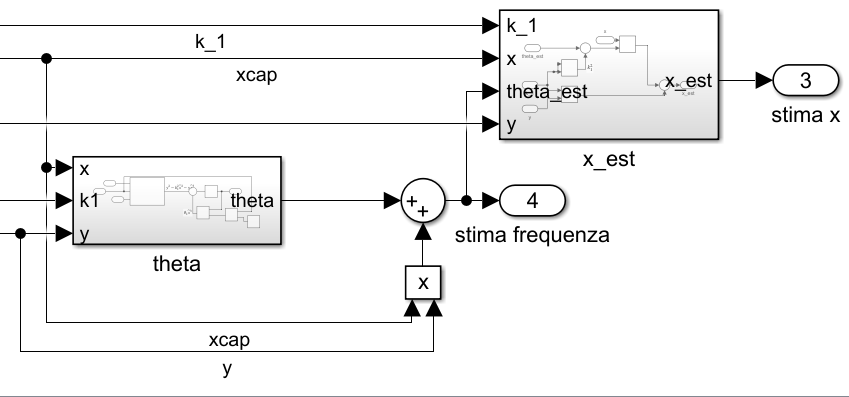
\includegraphics[scale=0.4]{2022-05-15-17-57-49.png} %chktex 8
        \end{figure}
    \end{minipage}
\end{frame}
\begin{frame}
    \frametitle{Simulink - 5} % chktex 8
    \subsection{Sistema Complessivo}
    \begin{figure}
            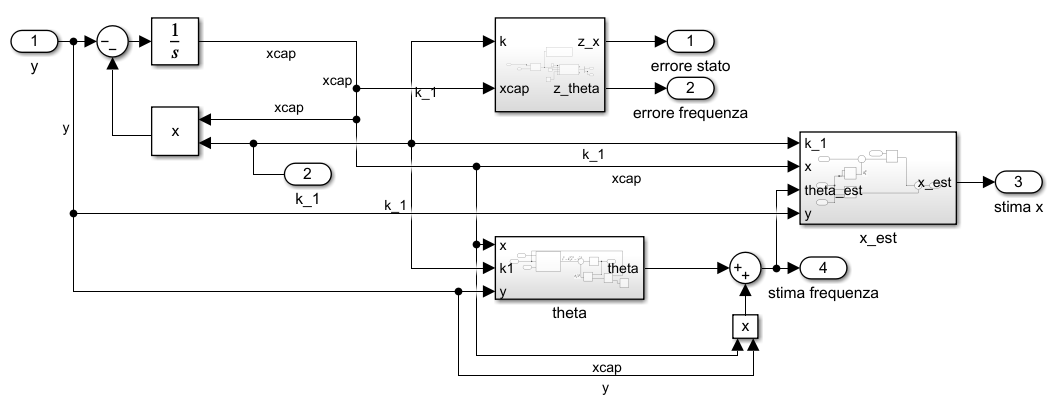
\includegraphics[scale=0.4]{2022-05-15-18-01-35.png} %chktex 8
        \end{figure}
\end{frame}
\begin{frame}
    \frametitle{\(y_{2}=\sin(t)\quad k_{1}=\{1,0.5,2\}\)}
    \section{Analisi}
    \subsection{\(y_{2}=\sin(t)\quad k_{1}=\{1,0.5,2\}\)}
    \begin{minipage}[t]{0.5\textwidth}
        \small
        Per \(k_{1}=0.5\) il tempo di convergenza dell'errore di stima della frequenza viene notevolmente ridotto; tuttavia l'errore di stima di \(x\) si allunga per poi convergere. Inoltre, l'andamento per k piccoli risultà più regolare.\\
        Per valori di \(k_{1}\) piccoli (nell'ordine di 0.01 circa) il tempo di convergenza aumenta (\>60s circa); per valori alti (nell'ordne di 100) la stima della frequenza non converge nel tempo di simulazione di 500s e il suo errore rimane pari ad 1. L'errore e la stima di x convergono.
    \end{minipage}\hspace{0.5cm}
    \begin{minipage}[t]{0.4\textwidth}
        \begin{figure}
            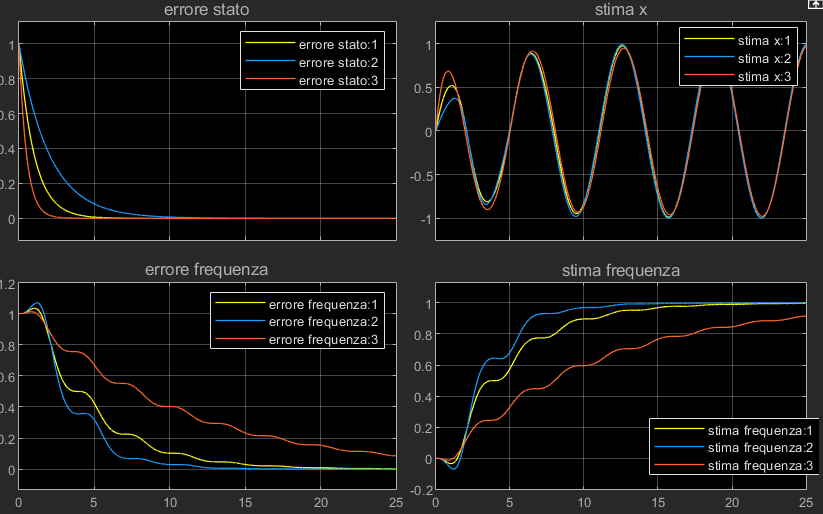
\includegraphics[scale=0.25]{2022-05-15-18-06-51.png}% chktex 8
            \caption{K=1 giallo, k=0.5 azzurro, k=2 marrone}
        \end{figure}
    \end{minipage}
\end{frame}
\begin{frame}
    \frametitle{\(y_{1}=\sin(100t)\quad k_{1}=\{1,0.5,2\}\)}
    \section{Analisi}
    \subsection{\(y_{1}=\sin(100t)\quad k_{1}=\{1,0.5,2\}\)}
    \begin{minipage}[t]{0.5\textwidth}
        \small
        Con \(y_{1}\) il tempo di convergenza viene notevolmente aumentato arrivando a \(8x10^{4}s\) circa. Ricordiamo che,la frequenza per questo segnale è \(\omega=100\) e la relazione che sussiste tra le due grandezze è \(\theta_{1}=\omega^2\) che è in accordo al grafico in figura.
    \end{minipage}\hspace{0.5cm}
    \begin{minipage}[t]{0.4\textwidth}
        \begin{figure}
            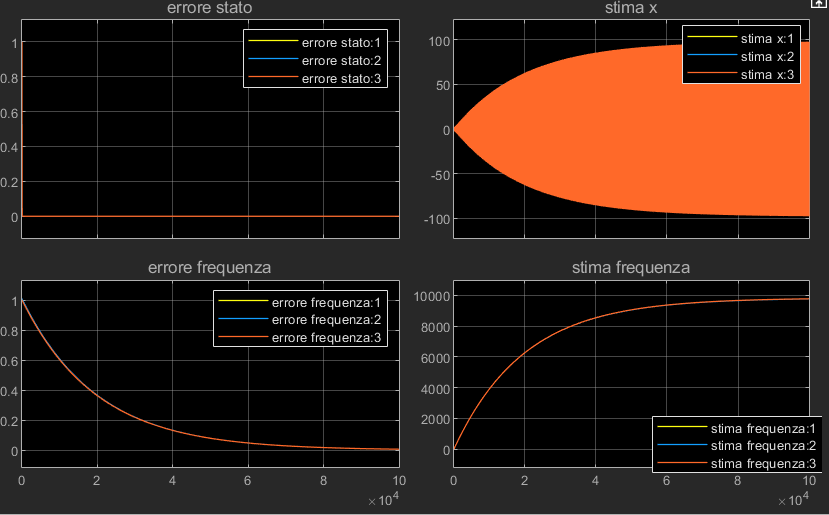
\includegraphics[scale=0.25]{2022-05-15-19-19-53.png}% chktex 8
            \caption{K=1 giallo, k=0.5 azzurro, k=2 marrone}
        \end{figure}
    \end{minipage}
\end{frame}
\begin{frame}
    \frametitle{Conclusioni}
    \section{Conclusioni}
    L'algoritmo I\&I dipende molto dalla frequenza del segnale di ingresso e dalla scelta del guadagno \(k_1\).\newline
    Una buona scelta del guadagno potrebbe essere in un intorno di 1.\newline
    Inoltre, questo approccio non risente notevolemnte del disturbo che abbiamo fornito in ingresso, ma risulta sensibile alle frequenze del segnale misurato dato che per \(y_2\) il tempo di convergenza era circa di 15s a confronto con quello per \(y_1\) di \(8x10^{4}s\) circa.
\end{frame}
\end{document}